\documentclass{beamer}
\usepackage{ccicons}
\usepackage{hyperref}
\usepackage{minted}

% ❤️ https://github.com/elauksap/focus-beamertheme
\usetheme{focus}
\title{Reactive Applications\\in Frontend Engineering Today}
\author{Manuel Alabor}
\institute{Master Seminar\\HSR University of Applied Sciences Rapperswil}
\date{}

\setminted{autogobble=true, tabsize=2, linenos=false, frame=none, breaklines=true}

\begin{document}

\begin{frame}
	\maketitle
	\Tiny{\ccby\thinspace\thinspace This work is licensed under a \href{https://creativecommons.org/licenses/by/4.0/}{Creative Commons Attribution 4.0 International License}}.
\end{frame}

% \begin{frame}{Overview}
% 	\tableofcontents
% \end{frame}

\section*{Welcome}

\begin{frame}{Motivation and Goals}
	\begin{itemize}
		\item Get \textbf{acquainted} with \textbf{scientific research work style}\bigskip
		\item \textbf{Review} a research report\bigskip
		\item \textbf{Transfer} topic to the \textbf{field} of \textbf{frontend engineering}\bigskip
		\item \textbf{Write} a research report\bigskip
	\end{itemize}
\end{frame}

\begin{frame}[focus]
	\emph{``On the Positive Effect of Reactive Programming on Software Comprehension: An Empirical Study''}
	\\\bigskip
	\small{Salvaneschi et al. \cite{7827078}}
\end{frame}


\subsection*{Research Questions}

\begin{frame}{RQ1: Design Sciences and \\Empirical Software Engineering}
	\begin{enumerate}
		\item[RQ1.1] Which \textbf{empirical research methods}, approaches and concepts \textbf{were applied} by Salvaneschi et al. \cite{7827078}?\bigskip
		\item[RQ1.2] Are these research methods, approaches and concepts \textbf{applied well}, what could have been done better?\bigskip
		\item[RQ1.3] \textbf{Do} Salvaneschi et al. \cite{7827078} \textbf{meet FAIR principles} \cite{2019arXiv190805986H} \cite{wilkinson:2016} with their work?
	\end{enumerate}
\end{frame}

\begin{frame}{RQ2: Software Engineering Principles}
	\begin{itemize}
		\item[RQ2.1] \textbf{How} do Salvaneschi et al. \cite{7827078} \textbf{define RP and OOP}?\bigskip
		\item[RQ2.2] \textbf{When} should \textbf{RP be considered}, and \textbf{when not}?\bigskip
		\item[RQ2.3] \textbf{Which experiments} should be \textbf{conducted in future} work?\bigskip
		\item[RQ2.4] \textbf{Which} design \textbf{alternatives exist} in the context of \textbf{frontend engineering}?
	\end{itemize}
\end{frame}


\section{Terminology}
\subsection*{Empirical Software Engineering}
\begin{frame}{Empirical Software Engineering}
	\begin{itemize}
		\item Lack of scientific and analytical formalism\bigskip
		\item Apply empirical research methods instead
	\end{itemize}
\end{frame}

\subsection*{Design Sciences}
\begin{frame}{Design Sciences \cite{wieringa}}
	\begin{itemize}
		\item Research \textbf{principle} to \textbf{grow} research \textbf{projects}\bigskip
		\item \textbf{Design} and \textbf{investigate} on \textbf{artifacts} in a specific \textbf{context}\bigskip
		\item \textbf{Iterate} until \textbf{stakeholders} are satisfied
	\end{itemize}

	\begin{figure}
		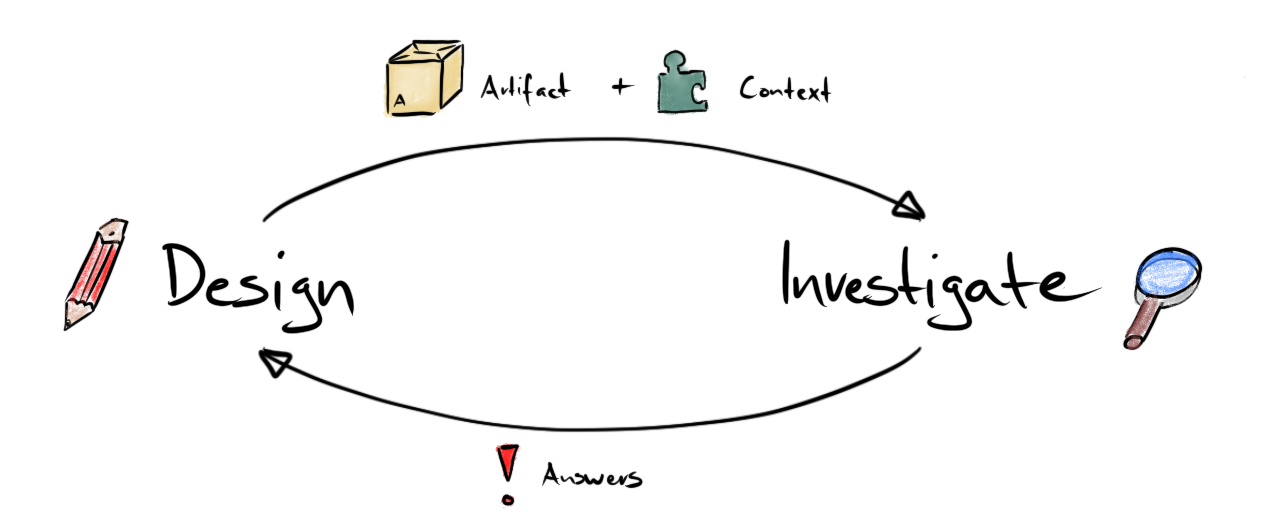
\includegraphics[width=.8\textwidth]{assets/slides/design-sciences-process.png}
	\end{figure}
\end{frame}

\subsection*{FAIR Research Principles}
\begin{frame}{FAIR Research Principles \cite{wilkinson:2016} \cite{2019arXiv190805986H}}
	\begin{itemize}
		\item \textbf{F}indability\bigskip
		\item \textbf{A}ccessibility\bigskip
		\item \textbf{I}nteroperability\bigskip
		\item \textbf{R}eusability
	\end{itemize}
\end{frame}

\subsection*{Reactive Programming}
\begin{frame}{Reactive Programming I}
	\begin{itemize}
		\item \textbf{Declarative} programming paradigm\bigskip
		\item Originated in functional programming\bigskip
		\item API to describe \textbf{values}, their \textbf{transformation} and how they \textbf{depend} on each other over time\bigskip
		\item \textbf{Runtime} environment maintaining \textbf{consistency}
	\end{itemize}
\end{frame}

\begin{frame}[fragile=singleslide]{Reactive Programming II}
	\textbf{TODO: Create Graphic}

	\begin{block}{Reactive Programming with BaconJS\footnote{\url{http://baconjs.github.io/}}}
		\begin{minted}{JavaScript}
			const currentDateString = Bacon
				.fromPoll(1000, () => new Date())
				.map(d => d.toISOString());
		\end{minted}
	\end{block}

\end{frame}

\subsection*{Observer Design Pattern}
\begin{frame}{Observer Design Pattern \cite{gamma1995design}}
	\begin{columns}[t, onlytextwidth]
		\column{0.5\textwidth}
			\begin{itemize}
				\item \textbf{Decouple} components while \textbf{maintaining communication} between them\bigskip
				\item Originated in object oriented programming\bigskip
			\end{itemize}

		\column{0.5\textwidth}
			\textbf{TODO Create Graphic}
	\end{columns}
\end{frame}



\section{Summary of Salvaneschi et al.}

\begin{frame}[focus]
	``\emph{(...) it has been repeatedly argued that RP greatly improves (...) comprehension of software.}''
	\\\bigskip
	\small{Salvaneschi et al. \cite{7827078}}
\end{frame}

\begin{frame}{Research Questions \cite{7827078}}
	\begin{itemize}
		\item \emph{``Does reactive programming \textbf{impact the correctness} of program comprehension?''}\bigskip
		\item \emph{``Does reactive programming \textbf{impact time} for program comprehension?''}\bigskip
		\item \emph{``Does comprehending RP programs \textbf{require a different programming skills level} than the OO style?''}\bigskip
		\item \emph{``What are the \textbf{reasons for a difference} - if any - in comprehending RP programs and OO programs?''}
	\end{itemize}
\end{frame}

\subsection*{Study Design}
\begin{frame}{Study Design}
	\begin{itemize}
		\item Subject \textbf{population} of a total of \textbf{127} students\bigskip
		\item Preparatory, quantitative programming \textbf{skill level survey}\bigskip
		\item \textbf{Controlled experiment} with two groups: RP vs. OOP\bigskip
		\item Quantitative/qualitative \textbf{survey} to collect \textbf{personal opinion}
	\end{itemize}
\end{frame}

\subsection*{Study Results}
\begin{frame}{Study Results}

	\begin{block}{Finding 1: \textbf{Correctness}}
		RP \textbf{increases} the \textbf{correctness} of program \textbf{comprehension}
	\end{block}
	\begin{block}{Finding 2: \textbf{Time}}
		RP style code \textbf{does not} require \textbf{more time} than comprehending its OOP equivalent
	\end{block}
	\begin{block}{Finding 3: \textbf{Skill Level}}
		RP code is \textbf{easier to understand} overall, \textbf{regardless} of the individuals programming \textbf{skill level}
	\end{block}
\end{frame}

\subsection*{Outlook}
\begin{frame}{Outlook}
	\begin{enumerate}
		\item \textbf{Interpretation} of collected results in context of \textbf{psychological research}\bigskip
		\item \textbf{Impact} of \textbf{language design} on RP \textbf{comprehensibility}\bigskip
		\item \textbf{Improvements} on \textbf{IDE support} for development of \textbf{reactive applications}
	\end{enumerate}
\end{frame}


\section{Review of Salvaneschi et al.}
\subsection*{Research Principle Score Card}
\begin{frame}{Research Principle Score Card}
	\begin{exampleblock}{Empirical Software Engineering}
		\begin{itemize}
			\item \textbf{Careful} study \textbf{setup} and \textbf{execution}
			\item \textbf{Transparent} description of \textbf{threats to validity}
		\end{itemize}
	\end{exampleblock}

	\begin{alertblock}{Design Sciences}
		\textbf{No evidence} for the \textbf{application} of \textbf{design sciences} found
	\end{alertblock}

	\begin{alertblock}{FAIR Research Principles}
		Lack of \textbf{complementary information} violates \textbf{Reusability} principle
	\end{alertblock}
\end{frame}

\subsection*{Software Engineering Score Card}
\begin{frame}{Software Engineering Score Card}
	\begin{exampleblock}{Reactive Applications}
		Introduction of classification schema: \textbf{Synthetic} and \textbf{interactive} applications, \textbf{graphical animations}
	\end{exampleblock}
	\begin{exampleblock}{Reactive Programming}
		\begin{itemize}
			\item Good overview noting \textbf{origins} in FP and \textbf{recent} development
			\item \textbf{Examples} using Scala
		\end{itemize}
	\end{exampleblock}

	\begin{alertblock}{Object Oriented Programming}
		\begin{itemize}
			\item \textbf{Limited overview} compared to RP
			\item \textbf{Reduced} to Observer Pattern, still \textbf{used synonymously}
		\end{itemize}
	\end{alertblock}
\end{frame}


\section*{Application in\texorpdfstring{\\}{ }Frontend Engineering}

\subsection*{Synthetic Application}
\begin{frame}{Synthetic Application: Scenario}
	\begin{columns}
		\column{0.6\textwidth}
			\begin{itemize}
				\item \textbf{Fetch} and \textbf{combine remote} profile and avatar \textbf{resource}\bigskip
				\item Avatar \textbf{depends} on profile resource\bigskip
			\end{itemize}

		\column{0.4\textwidth}
			\begin{block}{S1: \textbf{Modelling Data Flow}}
				\textbf{Fetch} a users \textbf{complete} profile \textbf{information} (name as well as their avatar picture) from \textbf{two} distinct \textbf{data sources}. The \textbf{profile} information \textbf{contains} required input to fetch the \textbf{avatar}. \textbf{Show} the combined information in the user interface \textbf{at once}.
			\end{block}
	\end{columns}
\end{frame}

\begin{frame}[fragile=singleslide]{Synthetic Application: Reactive Programming}
	\begin{block}{Modelling Data Flow with Promises}
		\begin{minted}{JavaScript}
			fetchProfile()
				.then(async (profile) => {
					const avatar = await fetchAvatar(profile);
					return { ...profile, ...avatar };
				})
				.then(renderUser);
		\end{minted}
	\end{block}
\end{frame}

\begin{frame}[fragile=singleslide]{Synthetic Application: Observer Pattern}
	\begin{block}{Modelling Data Flow with Observer Design Pattern \cite{gamma1995design} I}
		\begin{minted}{JavaScript}
			const profileObservable = observable();
			const avatarObservable = observable();
		\end{minted}
	\end{block}
\end{frame}

\begin{frame}[fragile=singleslide]{Synthetic Application: Observer Pattern}
	\begin{block}{Modelling Data Flow with Observer Design Pattern \cite{gamma1995design} II}
		\begin{minted}{JavaScript}
			profileObservable.addObserver(async () => {
				const a = await fetchAvatar(profileObservable.value);
				avatarObservable.value = a;
				avatarObservable.notify();
			});

			avatarObservable.addObserver(() => {
				renderUser({
					...profileObservable.value,
					...avatarObservable.value
				});
			});
		\end{minted}
	\end{block}
\end{frame}

\begin{frame}[fragile=singleslide]{Synthetic Application: Observer Pattern}
	\begin{block}{Modelling Data Flow with Observer Design Pattern \cite{gamma1995design} III}
		\begin{minted}{JavaScript}
			fetchProfile().then(profile => {
				profileObservable.value = profile;
				profileObservable.notify();
			});
		\end{minted}
	\end{block}
\end{frame}

\begin{frame}{Synthetic Application: Key Findings}
	\begin{itemize}
		\item \textbf{Key findings} in favor of reactive programming by Salvaneschi et al. \cite{7827078} \textbf{confirmed}:\smallskip
		\begin{itemize}
			\item \textbf{Less boilerplate} code\smallskip
			\item \textbf{Mental model} can be implemented \textbf{more accurately}
		\end{itemize}\bigskip
		\item \textbf{Reactive programming} is \textbf{better} suited for the implementation of \textbf{synthetic applications}
	\end{itemize}
\end{frame}

\subsection*{Interactive Application}
\begin{frame}[t]{Interactive Application}
	\begin{columns}[t]
		\column{0.5\textwidth}
			\begin{itemize}
				\item \textbf{Handle} user \textbf{interaction} with a user interface \textbf{component}
			\end{itemize}

		\column{0.5\textwidth}
			\begin{block}{S2: \textbf{Handle User Interaction}}
				Handle clicks on a button. \textbf{Every time} a \textbf{user clicks} the \textbf{button}, \textbf{log} the current \textbf{time}. The log shows a list of all user interactions eventually.
			\end{block}
	\end{columns}
\end{frame}

\begin{frame}[fragile=singleslide]{Interactive Application: Reactive Programming}
	\begin{block}{Handle User Interaction with BaconJS}
		\begin{minted}{JavaScript}
			Bacon.fromEvent(getButton(), "click")
				.map(() => new Date())
				.onValue(logInteraction);
		\end{minted}
	\end{block}
\end{frame}


\begin{frame}[fragile=singleslide]{Interactive Application: Observer Pattern}
	\begin{block}{Handle User Interaction with EventTarget Interface}
		\begin{minted}{JavaScript}
			getButton().addEventListener(
				"click",
				() => logInteraction(new Date())
			);
		\end{minted}
	\end{block}
\end{frame}

\begin{frame}{Interactive Application: Key Findings}
	\begin{itemize}
		\item \textbf{Both} solutions have similar \textbf{small code footprint}\bigskip
		\item \textbf{Reactive programming} variation introduces \textbf{hidden complexity}\bigskip
		\item \textbf{Do not use} any paradigm simply \textbf{for the sake of it}
	\end{itemize}
\end{frame}

\subsection*{Criteria Catalog}
\begin{frame}[focus]
	When Should I\\Use What?!
\end{frame}

\begin{frame}[fragile=singleslide]{Criteria Catalog}
	\begin{figure}
		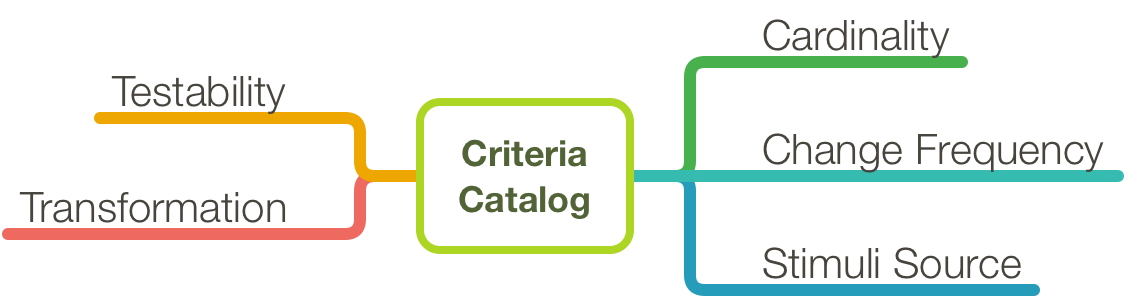
\includegraphics[width=\textwidth]{assets/slides/criteria-catalog.png}
	\end{figure}
\end{frame}

\section{Outlook}
\begin{frame}{Future Research Suggestions}
	\begin{enumerate}
		\item \textbf{Verify} presented \textbf{scenarios} and \textbf{criteria catalog} in an empirical study\bigskip
		\item \textbf{Explore W3C Web Animation API} draft for more complex, high-performance animation behaviors\bigskip
		\item Research to \textbf{improve} development \textbf{tool support} for \textbf{reactive programming}
	\end{enumerate}
\end{frame}


\section{Conclusion}
\begin{frame}{Recap}
	\begin{itemize}
		\item \textbf{Summary and review} on paper by Salvaneschi et al. \cite{7827078}\bigskip
		\item \textbf{Transferred} results by Salvaneschi et al. \textbf{to} context of \textbf{frontend engineering}\bigskip
		\item \textbf{Suggested three} potential \textbf{topics} for future research
	\end{itemize}
\end{frame}

\begin{frame}
	\begin{center}
		\emph{We selected ``Research to improve development tool support for reactive programming'' as topic for our own future research.}
	\end{center}
\end{frame}

\begin{frame}[focus]
	Questions?
\end{frame}

\begin{frame}[focus]
	Discussion
\end{frame}

\appendix
\begin{frame}[allowframebreaks]{References}
	\bibliographystyle{plain}
	\bibliography{bibliography}
\end{frame}

\end{document}